\documentclass{letask}
\usepackage{gnuplottex}
\usepackage{epstopdf}
\usepackage{enumitem}
\setlist{resume, leftmargin=0cm, topsep=0cm, resume}
\usepackage{iunits}

\begin{document}
\begin{titlepage}
\center % Center everything on the page
 
%----------------------------------------------------------------------------------------
%	HEADING SECTIONS
%----------------------------------------------------------------------------------------

\textsc{\LARGE Московский\\[-0.2cm]Физико-Технический Институт\\[0.1cm]\large (государственный университет)}\\[1.5cm] % Name of your university/college
\textsc{\Large Кафедра общей физики}\\[0.1cm] % Major heading such as course name
\textsc{\large Вопрос по выбору, 3 семестр}\\[0.5cm] % Minor heading such as course title

%----------------------------------------------------------------------------------------
%	TITLE SECTION
%----------------------------------------------------------------------------------------

\HRule
\\[0.8cm]
{ \huge \bfseries Исследование работы импульсного\\[0.1cm] преобразователя напряжения}
\\[0.8cm] % Title of your document
\HRule
\\[1.5cm]


 
%----------------------------------------------------------------------------------------
%	AUTHOR SECTION
%----------------------------------------------------------------------------------------

\begin{minipage}{0.4\textwidth}
	\begin{flushleft} \large
		\textsf{Студент}
		
		Георгий \textsc{Корепанов} \\[-0.15cm]
		512 группа
	\end{flushleft}
\end{minipage}
~
\begin{minipage}{0.4\textwidth}
	\begin{flushright} \large
		\textsf{Преподаватель}
		
		Виктор Иванович \\[-0.15cm]
		\textsc{Чивилёв} % Supervisor's Name
	\end{flushright}
\end{minipage}

\begin{bottompar}
	\begin{center}
		
\includegraphics[width = 80 mm]{logo.jpg}
	\end{center}
	{\large \today}

\end{bottompar}
\vfill % Fill the rest of the page with whitespace

\end{titlepage}



\section{Введение}

В практике радиолюбителей часто возникает задача преобразования постоянного напряжения (DC $\rightarrow$ DC). Трансформаторные преобразователи сложны схемотехнически и требуют тонкого расчёта. Появление \textbf{импульсных} преобразователей перевернуло мир источников питания --- современные адаптеры для мобильных телефонов легко помещаются в кармане.

В данной работе рассмотрена интересная идея преобразования постоянного напряжения, позволяющая относительно просто изготовить преобразователь, работающий в широком диапазоне напряжений (напряжение батарейки \textbf{AA} можно легко конвертировать до величин порядка \textbf{$\mathbf{500}$ и более вольт}).


\section*{Идея получения высокого напряжения}
Создадим начальный ток в катушке, замкнув ею источник и землю. Затем размыканием ключа изменим направление течения тока, <<отправив>> его на конденсатор ёмкостью $C = 10~\mk\F$:
\begin{figure}[H]
\begin{minipage}[h]{0.49\linewidth}
\centering
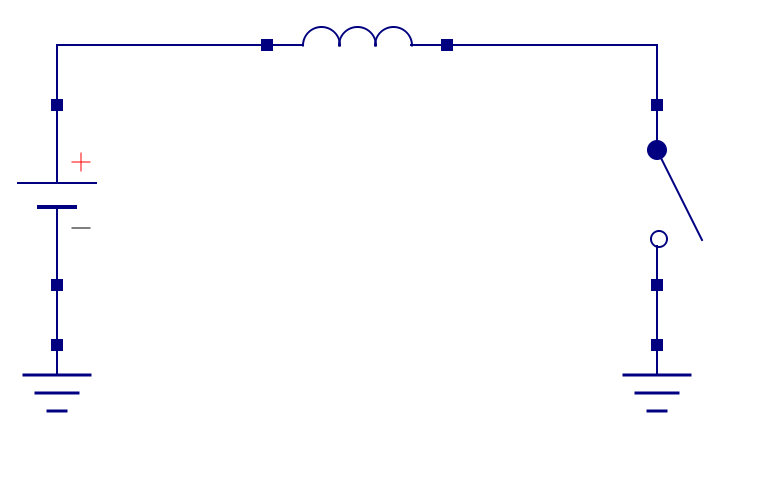
\includegraphics[height=.4\textwidth]{c-1.png}
\caption{Создание начального тока}
\end{minipage}
\hfill
\begin{minipage}[h]{0.49\linewidth}
\centering
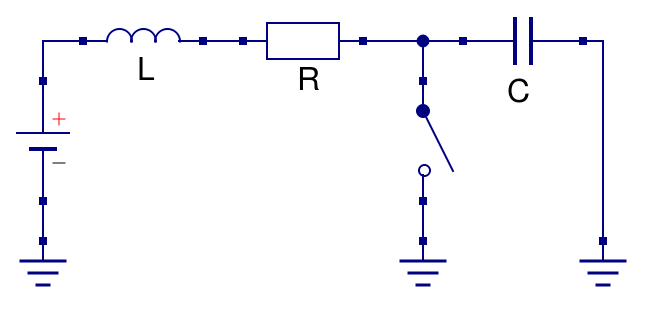
\includegraphics[height=.4\textwidth]{c-4.png}
\caption{Подключение конденсатора}
\end{minipage}
\end{figure}


\vspace{-1em}
\section*{Первые расчёты}
Сразу перейдём к практике. Здесь и далее используется источник постоянного напряжения с $U_0 = 10~\V$.

Реальные катушки имеют конечное активное сопротивление. Будем рассматривать катушку с $R = 1~\Ohm$ и $L = 200~\H$ (вполне типичные параметры для катушки с сердечником, подходящим для работы в режиме преобразования напряжения); введём обозначение для характерного времени установления тока в катушке: $\tau \equiv L/R$.
\begin{figure}[H]
\centering
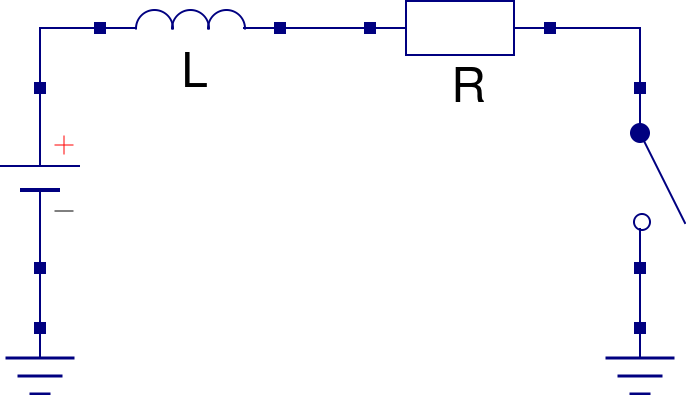
\includegraphics[width = 0.38\textwidth]{c-2.png}
\caption{Эквивалентная схема с активным сопротивлением катушки}
\end{figure}

При возбуждении в катушке некоторого тока часть энергии рассеивается на резисторе, поэтому нет смысла держать ключ открытым слишком долгое время. Выясним, как эти потери зависят от времени.

Для создания преобразователя используем микросхему MAX1771, работающую на частоте $\nu = 300~\k\Hz$. Следовательно, вычисления следует проводить для времён открытия ключа $~\sim~ t_\text{пр} = 1/\nu \ll \tau$). Это позволит существенно упростить расчёты.

\begin{enumerate}
\item Найдём зависимость $I(t)$ тока, текущего через катушку, от времени с момента включения. Операторный коэффициент передачи
\begin{align*}
K(p) &= \frac{R}{pL+R} \quad\Rightarrow\\
\Rightarrow\quad
I(t) &= U_R(t)/R \risingdotseq\frac{1}{R}\mathcal{L}(U(t)) = \frac{1}{p(p+R/L)} \risingdotseq \frac{U_0}{R} \left(1-e^{-t/\tau}\right) \simeq \frac{U_0}{R} \frac{t}{\tau}.
\end{align*}

\item После размыкания ключа процессы в цепи описываются обыкновенным дифференциальным уравнением второго порядка для LRC-цепочки. Имеем
$$LC \ddot U +R \dot U + U = U_0,$$
где $U$~--- напряжение на конденсаторе. Общее решение данного уравнения квазипериодично (затухающие колебания):
\begin{figure}[H]
\centering
\caption{Качественный график решения при $U(0) = U_0$}
\begin{gnuplot}[terminal=epslatex]
set samples 10000
set xrange [0:10]
set yrange [9:11]
set ylabel "$U$, \\V"
set xlabel "$t$, \\ms"
set key off
set grid
set size 1.25,1.17
f(x) = 10*(0.1*sin(3*x)*exp(-x*0.3)+1)
plot f(x) lw 3 lc 6
\end{gnuplot}
\end{figure}

Видно, что после размыкания ключа напряжение на конденсаторе превышает $U_0$. Если в схему добавить диод, напряжение на конденсаторе <<зафиксируется>> на максимальном значении.
\begin{figure}[H]
\centering
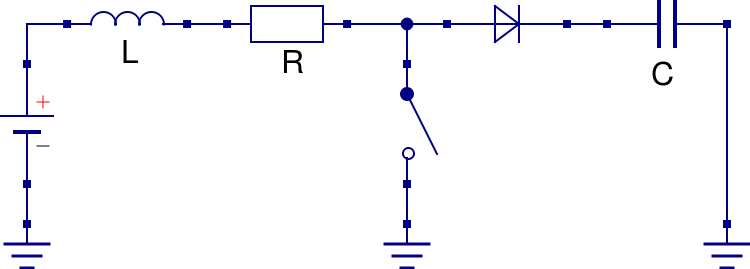
\includegraphics[width = 0.6\textwidth]{c-5.png}
\caption{Схема с добавленным диодом}
\end{figure}
\end{enumerate}


\section*{Большие напряжения}

\begin{enumerate}
\item Положим начальное напряжение на конденсаторе достаточно большим: $U_C = 100~\V$. Это упрощает исследование решения полученного дифференциального уравнения, поскольку скачок напряжения $U_\text{ск} \ll U_C$. 

Проверим последнее утверждение. Введём замену $\varphi \equiv U-U_0$:
$$\ddot \varphi + 2\gamma \dot \varphi + \omega_0^2 \varphi = 0,$$
где обыкновенно $\omega_0^2 = 1/LC$, $\gamma = R/2L$.
\begin{figure}[H]
\centering
\caption{Качественный график решения при $U(0) = U_C$}
\begin{gnuplot}[terminal=epslatex]
set samples 10000
set xrange [0:10]
set yrange [-100:100]
set ylabel "$U$, \\V"
set xlabel "$t$, \\ms"
set key off
set grid
set size 1.25,1.17
f(x) = 100*cos(3*x-0.6)*exp(-x*0.3)
plot f(x) lw 3 lc 6
\end{gnuplot}
\end{figure}

При условии $\Delta t \ll T$ в разложении решения в ряд Тейлора в точке максимума $t_0$ можно ограничиться производной второго порядка:
$$\varphi(t_0+\Delta t) \simeq \varphi(t_0) + \cancelto{\scriptstyle 0}{\dot \varphi(t_0) \Delta t}~~+ \frac12\, \ddot \varphi(t_0) \Delta t^2.$$
Учитывая, что в максимуме $\ddot \varphi =  - \omega_0^2 \varphi(t_0)$, $\varphi(t_0) = \varphi(0)+U_\text{ск}$, $\dot \varphi (0) \simeq - \ddot \varphi \Delta t$, а также $I = C \dot \varphi$, имеем
$$\Delta t = \frac{LI}{\varphi(0)}, \quad U_\text{ск} = I^2 \frac{L}{2C} \frac{1}{\varphi(0)},$$
причём из условия $\Delta t  \ll T$ следует 
$$I \ll \varphi(0) \sqrt{C/L}.$$

\item Проверим, что последнее соотношение выполнено даже для максимально возможного тока в катушке (время возбуждения тока в катушке равно $t_\text{пр}$):
$$I_{\max} = \frac{U_0}{R} \frac{t_\text{пр}}{\tau} = 0,17~\A, \quad \varphi(0) \sqrt{C/L} = 20,1~\A$$ 
\end{enumerate}


\section*{Реальный преобразователь}

Чтобы осуществлять дальнейшее повышение напряжения, необходимо периодически замыкать и размыкать ключ: напряжение на конденсаторе будет расти скачками, хотя, очевидно, скачки будут тем слабее, чем больше напряжение на конденсаторе. В реальном преобразователе эту работу выполняет специализированная микросхема.

\subsection*{Расчёт работы преобразователя}

Пусть на конденсаторе установилось напряжение $U_C = 100~\V$: через \emph{подключённую параллельно конденсатору} нагрузку течет ток, компенсирующий рост напряжения в результате работы схемы преобразователя.

Ключ замыкается на время $t_L$, размыкается на $(t_\text{пр} - t_L)$~--- имеем меандр со скважностью $s = t_L/t_\text{пр}$:

\begin{figure}[H]
\centering
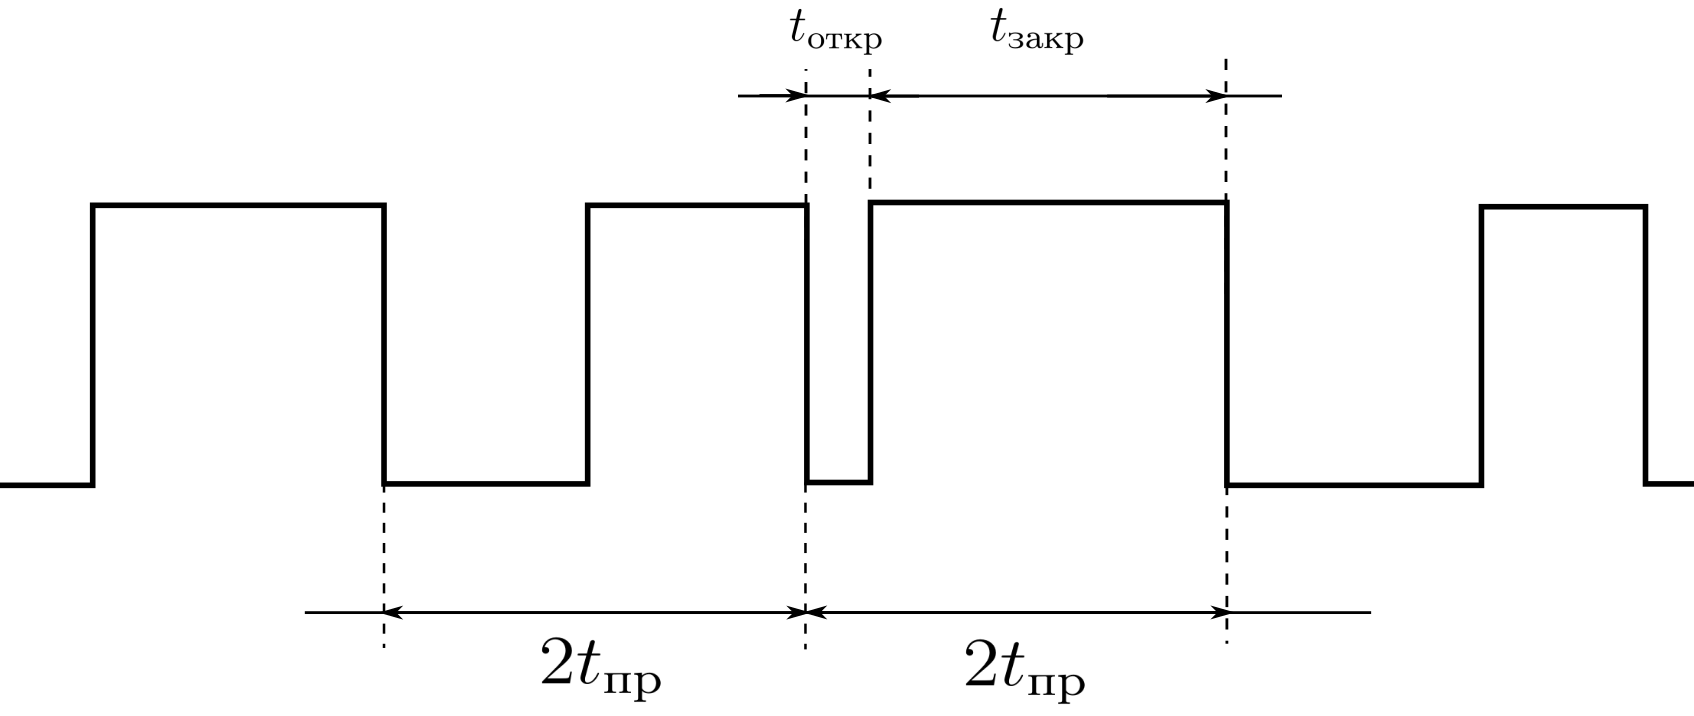
\includegraphics[width = 0.9\textwidth]{c-6.png}
\caption{График меандра переменной скважности}
\end{figure}

\begin{enumerate}

\item Будем считать, что скважность сигнала не слишком велика, так что $t_0 < t_\text{пр} - t_L$. Последнее верно при скважности, меньшей, чем 
$$ s_{\max} = \frac{1}{1+U_0/\varphi(0)} = 0,9.$$
\end{enumerate}


\section*{Стабилизация напряжения}

Преобразователь должен подстраиваться под значение тока в нагрузке, стабилизируя напряжение на выходе; в противном случае либо мощности будет не хватать, и заряд с конденсатора быстро стравится в нагрузку, либо преобразователь будет нагнетать слишком большое напряжение на выходе.

Для этого при уменьшении тока нагрузки уменьшается скважность меандра, управляющего ключом. Тогда за период работы преобразователя в катушке возбуждается меньший ток, и конденсатору передается меньшая энергия. В пределе, когда нагрузка отключена, а утечки конденсатора пренебрежимо малы, скважность сигнала стремится к 100\% (ключ всегда закрыт, ток не течет).

\begin{enumerate}
\item Найдём зависимость скважности сигнала меандра от тока нагрузки:
$$U_\text{ск} = \frac{\Delta q}{C}=  \frac{\left< I \right> t_\text{пр}}{C}
\quad\Rightarrow\quad
\left< I \right> = \frac{CU_\text{ск}}{t_\text{пр}} = \frac{s^2}{\nu} \frac{U_0}{U_\text{вых}-U_0} \frac{U_0}{2L}.$$
Производя расчёты, получим 
$$I = s^2 \cdot 9,3~\m\A,$$
то есть максимальный ток нагрузки
$$I_{\max} = 0,9^2 \cdot 9~\m\A = 7,5~\m\A.$$
\end{enumerate} 


\section*{Мощность и КПД преобразователя}

\begin{enumerate}
\item По выходным току и напряжению возможно рассчитать выходную мощность:
$$W = \frac{s^2}{\nu} \frac{U_0 U_\text{вых}}{U_\text{вых}-U_0} \frac{U_0}{2L} \simeq \Big| U_0 \ll U_\text{вых} \Big| \simeq \frac{s^2}{\nu} \frac{U_0^2}{2L}.$$
Видно, что увеличение индуктивности катушки и/или частоты преобразования ведёт к уменьшению выходной мощности преобразователя. Однако повысить мощность, уменьшив эти величины, на практике затруднительно, поскольку уменьшение их обеих ведёт к увеличению максимального тока, протекающего по катушке:
$$I_{\max} = \frac{U_0}{\nu L}.$$
Таким образом, можно заключить, что <<чудес не бывает>>: при попытке увеличить мощность преобразователя мы сталкиваемся с непреодолимой физической трудностью, заключающейся в необходимости увеличивать максимальный ток катушки, что приводит к увеличению её размеров, и, как следствие, к увеличению размеров конечного устройства. Более совершенные схемы позволяют в какой-то степени обойти это ограничение, однако его общий характер сохраняется (так, например, блок питания ноутбука всегда значительно больше блока питания телефона). 
\end{enumerate}

\subsection*{КПД преобразователя}
\begin{enumerate}
\item Практически важным вопросом является расчёт КПД преобразователя. Выходная мощность уже известна. Найдём работу источника.
Работа по возбуждению тока в~катушке
$$A_1 = \int_0^t U_0 I \,dt = \frac{U_0^2}{\nu^2} \frac{s^2}{2L}.$$
Работа источника после размыкания ключа
$$A_2 = U_0 \,\Delta q = U_0 \cdot C U_\text{ск} = \frac{U_0 \left< I \right>}{\nu} = \frac{s^2}{\nu^2} \frac{U_0^2}{U_\text{вых}-U_0} \frac{U_0}{L}.$$
Полная мощность источника
$$W_\text{ист} = \frac{A_1+A_2}{t_\text{пр}} = \frac{U_0^2}{\nu} \frac{s^2}{2L} \left( 1+ \frac{2U_0}{U_\text{вых} - U_0} \right).$$
\item Окончательно получаем для КПД системы
$$\eta = \frac{W}{W_\text{ист}} = \left( 1+\frac{2U_0}{U_\text{вых}-U_0} \right)^{-1} \frac{U\text{вых}}{U_\text{вых}-U_0} = \left( 1+\frac{U_0}{U_\text{вых}} \right)^{-1} \simeq \Big| U_0 \ll U_\text{вых} \Big| \simeq 1.$$

Мы получили примечательное соотношение, показывающее, что КПД импульсного преобразователя сверху ограничен \emph{только} единицей, и не падает (а, согласно полученному результату, даже растёт) с ростом разницы напряжений. Этот вывод, конечно, не учитывает прочих потерь в схеме, которые, вообще говоря, растут с ростом напряжения, но он показывает, что для КПД преобразователя нет \textbf{принципиальных} ограничений сверху.
\end{enumerate}


\section*{Пара слов о существующих схемах}

\begin{figure}[H]
\begin{minipage}[h]{0.49\linewidth}
\centering
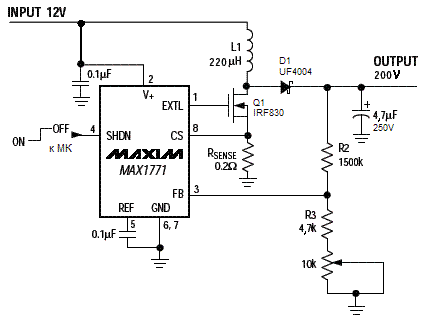
\includegraphics[height=.7\textwidth]{c-7.png}
\caption{Принципиальная схема}
\end{minipage}
\hfill
\begin{minipage}[h]{0.49\linewidth}
\centering
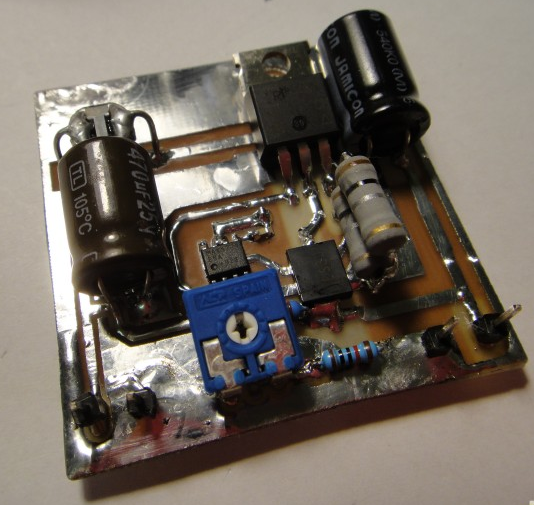
\includegraphics[height=.7\textwidth]{c-8.png}
\caption{Cобранный преобразователь}
\end{minipage}
\end{figure}

\begin{enumerate}
\item В схеме, кроме указанных выше элементов, присутствуют два дополнительных: резистор $R_\text{SENSE}$, по напряжению на котором определяется и ограничивается максимальный ток в цепи, предохраняя преобразователь от короткого замыкания и перенагрузки, и резисторный делитель $R2-R3-10\mathrm{k}$, с помощью которого микросхема <<определяет>> напряжение на выходе преобразователя.
\end{enumerate}


\section*{Экспериментальная часть}
Для проверки теоретических результатов снимем зависимость $I(s)$ и измерим КПД преобразователя, подключая к выходу преобразователя потенциометр и варьируя его сопротивление.

\subsection*{Измерение зависимости тока от скважности сигнала}

\begin{figure}[H]
\centering
\begin{gnuplot}[terminal=epslatex]
set samples 10000
set xrange [0:1]
set yrange [0:18]
set ylabel "$I,$ \\m\\A"
set xlabel "$s$"
set key off
set grid
set size 1.1,1.0

f(x) = 17*(x**2)/(0.8**2)
plot "data1.dat" using 2:1 ps 3 pt 7 lc 6, f(x) lc 6 lw 5
\end{gnuplot}
\caption{Аппроксимация полученной зависимости параболой}
\end{figure}

\begin{figure}[H]
\centering
\begin{gnuplot}[terminal=epslatex]
set samples 10000
set xrange [0:0.8]
set yrange [0:18]
set ylabel "$I,$ \\m\\A"
set xlabel "$s^2$"
set key off
set grid
set size 1.1,1.0

f(x) = a*x
fit f(x) "data2.dat" using 2:1 via a
plot "data2.dat" using 2:1 ps 3 pt 7 lc 6, f(x) lc 6 lw 5
\end{gnuplot}
\caption{Лианеризованная зависимость}
\end{figure}

\subsection*{Измерение КПД}
\begin{table}[H]
\centering
\begin{tabular}{|c|c|c|c|c|}
\hline
$I_\text{вх},~\m\A$ & $U_\text{вх},~\V$ & $I_\text{вых},~\m\A$ & $U_\text{вых},~\V$ & $\eta,~\%$ \\ \hline
22,8          & 12,0          & 2              & 182                  & 75        \\ \hline
35,0          & 12,0          & 3              & 182                  & 77        \\ \hline
57,6          & 12,0          & 5              & 182                  & 76        \\ \hline
72,8          & 12,0          & 6              & 182                  & 80        \\ \hline
98,2          & 12,0          & 8              & 182                  & 81        \\ \hline
124,4         & 12,0          & 10             & 182                  & 82        \\ \hline
195,9         & 12,0          & 15             & 182                  & 86        \\ \hline
\end{tabular}
\caption{Измерение КПД при разных нагрузках}
\end{table}

Заметно, что в силу особенностей работы схемы проявляется зависимость КПД от тока в нагрузке. Выявить явный вид этой зависимости не удаётся, однако теоретическую оценку среднего значения КПД можно считать оправданной (разумеется, она завышена, поскольку не были учтены ни питание микроконтроллера, ни дополнительные потери в катушке, ни утечки конденсатора, ни даже потери в ключевом транзисторе):
$$\left< \eta \right> \approx (80 \pm 6)\,\%,$$
$$\eta_\text{теор} = 93\,\%.$$

\section*{Результаты}
\begin{enumerate}[itemsep=0cm]
\setcounter{enumi}{0}
\item Успешно разработана схема преобразователя.
\item Схема реализована на монтажной плате и протестирована.
\item Исследован принцип работы схемы.
\item Из физических соображений получены важные зависимости, имеющие значение при разработке преобразователей.
\item Данные зависимости проверены экспериментально.
\end{enumerate}

\end{document}